%%%%%%%%%%%%%%%%%%%%%%%%%%%%%%%%%%%%%%%
%                                                                              
% 	Latex Vorlage  
%                                                                              
%%%%%%%%%%%%%%%%%%%%%%%%%%%%%%%%%%%%%%%

%%%%%%%%%%%%%%%%%%%%%%%%%%%%%%%%%%%%%%%
%                                                                              
% 	PREEMBLE  
%                                                                              
%%%%%%%%%%%%%%%%%%%%%%%%%%%%%%%%%%%%%%%

%
% Legt die Grundstruktur bzw. die Art des Dokuments sowie die Standardschriftgröße fest. 
%
\documentclass[12pt]{article}

%
% Legt das Seitenlayout fest.
%
\usepackage[a4paper, margin=1.0in]{geometry}

%
% Legt die verwendete Schrift fest.
%


%
% Legt die Worttrennungsregeln fest.
%
\usepackage[ngerman]{babel}

%
% Legt die Eingabekodierung fest.
%
\usepackage[utf8]{inputenc}
\usepackage[T1]{fontenc}

%
% Ermöglicht die Darstellung von Farben sowie die Bezeichnung von Farben durch Namen.
%
\usepackage[usenames, dvipsnames]{color}

%
% Ermöglicht das Einfügen von Grafiken.
%
\usepackage{graphicx}

%
% Erleichtert die Darstellung von URLs.
%
\usepackage{url}

%
% Erlaubt die Bearbeitung von Bilder-, Diagramm- und Tabellenunterschriften.
%
\usepackage[hang, normalsize, bf]{caption}

%
% Legt fest, dass die AMS-Symbole benutzt werden.
%
\usepackage{amsmath}
\usepackage{amssymb}

%
% Ermöglicht die Verwendung von vielen mathematischen Symbolen.
%
% \usepackage{mathabx}

%
% Ermöglicht die Verwendung der \today-Anweisung.
%
\usepackage[nodayofweek]{datetime}

% Erleichtert die Formattierung von Quelltexten.
\usepackage{listings}

%
% Ermöglicht die einfachere Bearbeitung von Tabellen.
%
\usepackage{tabularx}

%
% Ermöglicht die Darstellung von Tabellen auf mehreren Seiten (s. Dokumentation). 
%
\usepackage{ltxtable}

%
% Ermöglicht, Appendices in das Inhaltverzeichnis zu übernehmen.
%
\usepackage[toc]{appendix}

%
% Ermöglicht das Zusammenfügen mehrerer Zeilen einer Tabelle.
%
\usepackage{multirow}

%
% setzt Leerzeichen, wenn welche hingehören (vor nächstem wort, aber nicht vor "." oder ")")
%
\usepackage{xspace} 

%
% Legt fest, welche Sprache in der Bibliographie verwendet werden soll.
%
\usepackage[fixlanguage]{babelbib}

%%%%%%%%%%%%%%%%%%%%%%%%%%%%%%%%%%%%%%%%%%%%%%%%%%%%%%%%%%%%%%%%%%%%%%%%%%%%%%%%
%                                                                              
% 			Einstellungen                                                                
%                                                                              
%%%%%%%%%%%%%%%%%%%%%%%%%%%%%%%%%%%%%%%%%%%%%%%%%%%%%%%%%%%%%%%%%%%%%%%%%%%%%%%%

%%%%%%%%%%%%%%%%%%%%%%%%%%%%%%%%%%%%%%%%%%%%%%%%%%%%%%%%%%%%%%%%%%%%%%%%%%%%%%%%			
%	einstellungen: url
%%%%%%%%%%%%%%%%%%%%%%%%%%%%%%%%%%%%%%%%%%%%%%%%%%%%%%%%%%%%%%%%%%%%%%%%%%%%%%%%

\urlstyle{tt}

%%%%%%%%%%%%%%%%%%%%%%%%%%%%%%%%%%%%%%%%%%%%%%%%%%%%%%%%%%%%%%%%%%%%%%%%%%%%%%%%
% einstellungen: bibliographie
%%%%%%%%%%%%%%%%%%%%%%%%%%%%%%%%%%%%%%%%%%%%%%%%%%%%%%%%%%%%%%%%%%%%%%%%%%%%%%%%

\selectbiblanguage{german}
\bibliographystyle{babplain}

%%%%%%%%%%%%%%%%%%%%%%%%%%%%%%%%%%%%%%%%%%%%%%%%%%%%%%%%%%%%%%%%%%%%%%%%%%%%%%%%
%                                                                              
% 			ANWEISUNGEN                                                                  
%                                                                              
%%%%%%%%%%%%%%%%%%%%%%%%%%%%%%%%%%%%%%%%%%%%%%%%%%%%%%%%%%%%%%%%%%%%%%%%%%%%%%%%

%%%%%%%%%%%%%%%%%%%%%%%%%%%%%%%%%%%%%%%%%%%%%%%%%%%%%%%%%%%%%%%%%%%%%%%%%%%%%%%%
% anweisungen: römische zahlen
%%%%%%%%%%%%%%%%%%%%%%%%%%%%%%%%%%%%%%%%%%%%%%%%%%%%%%%%%%%%%%%%%%%%%%%%%%%%%%%%

\makeatletter
\newcommand{\rmnum}[1]{\romannumeral #1}
\newcommand{\Rmnum}[1]{\expandafter\@slowromancap\romannumeral #1@}
\makeatother

%%%%%%%%%%%%%%%%%%%%%%%%%%%%%%%%%%%%%%%%%%%%%%%%%%%%%%%%%%%%%%%%%%%%%%%%%%%%%%%%
%
% 			TEMPLATES
%
%%%%%%%%%%%%%%%%%%%%%%%%%%%%%%%%%%%%%%%%%%%%%%%%%%%%%%%%%%%%%%%%%%%%%%%%%%%%%%%%

%%%%% links - rechtsbuendig
%
%	\begin{flushleft}
%
%	\end{flushleft}
%
%
%

%%%%%%%%%%%%%%% BILDER IMPORTIEREN %%%%%%%%%%%%%%%%
%
%		\scalebox{0.45}{\includegraphics{data/fig/ganth_Diagramm.png}}

            
%%%%%%%%%%%%%%% Tabelle %%%%%%%%%%%%%%%% 
%
%        \large    
%        \begin{tabularx}{\textwidth}{ l l X }
%            
%            \emph{Autoren}:     &                   & \emph{Betreuer}:             \\
%                                &                   &                              \\
%            Hady Khalifa 				& (Mat-Nr.\ 123123) &	Computervisualstik und Design    \\
%            
%
%        \end{tabularx}
%            
%        \vfill
%        {\Large \today}
%        \end{center}


%%%%%%%%%%%%%%%%%%%%%%%%%%%%%%%%%%%%%%%%%%%%%%%%%%%%%%%%%%%%%%%%%%%%%%%%%%%%%%%%
%                                                                              
% 			DOKUMENT                                                                     
%                                                                              
%%%%%%%%%%%%%%%%%%%%%%%%%%%%%%%%%%%%%%%%%%%%%%%%%%%%%%%%%%%%%%%%%%%%%%%%%%%%%%%%

\begin{document}

%%%%%%%%%%%%%%%%%%%%%%%%%%%%%%%%%%%%%%%%%%%%%%%%%%%%%%%%%%%%%%%%%%%%%%%%%%%%%%%%
% dokument: titelblatt
%%%%%%%%%%%%%%%%%%%%%%%%%%%%%%%%%%%%%%%%%%%%%%%%%%%%%%%%%%%%%%%%%%%%%%%%%%%%%%%%

\begin{titlepage}

        %
        % CVD-Logo
        %
        
        \begin{center}
        
\includegraphics[scale=0.15, keepaspectratio=true]{data/fig/CVD_Logo.png}
        \end{center}
        
       

        %
        % university, department & lecture info
        %
        
        \begin{center}
            
            
            {\huge \bfseries
            		\ \\
            		\ \\
            		\ \\
            		\ \\
            		\ \\
            		\ \\
                Pflichtenheft\\
				Name des Projekts\\
				Eindeutige Teamnummer\\
				Datum\\
				\ \\
				\ \\
			
            }
            
		\end{center}


\end{titlepage}

%%%%%%%%%%%%%%%%%%%%%%%%%%%%%%%%%%%%%%%%%%%%%%%%%%%%%%%%%%%%%%%%%%%%%%%%%%%%%%%%
% dokument: inhaltsverzeichnis
%%%%%%%%%%%%%%%%%%%%%%%%%%%%%%%%%%%%%%%%%%%%%%%%%%%%%%%%%%%%%%%%%%%%%%%%%%%%%%%%

%
% Festlegung Art der Zitierung - Havardmethode: Abkuerzung Autor + Jahr
%
\bibliographystyle{alphadin}

\tableofcontents{}
\newpage{}

%%%%%%%%%%%%%%%%%%%%%%%%%%%%%%%%%%%%%%%%%%%%%%%%%%%%%%%%%%%%%%%%%%%%%%%%%%%%%%%%
% dokument: kapitel
%%%%%%%%%%%%%%%%%%%%%%%%%%%%%%%%%%%%%%%%%%%%%%%%%%%%%%%%%%%%%%%%%%%%%%%%%%%%%%%%


\section{Management- und Dokumentationsattribute}

       
	\noindent %%%%%%%%%%%%%%%%%%%%%%%%%%%%%%%%%%%%%%%
%                                                                              
% 		Management- und Dokumentationsattribute 			      		
%                                                                              
%%%%%%%%%%%%%%%%%%%%%%%%%%%%%%%%%%%%%%%

TODO Einleitung Management- und Dokumentationsattribute\\
\scalebox{0.45}{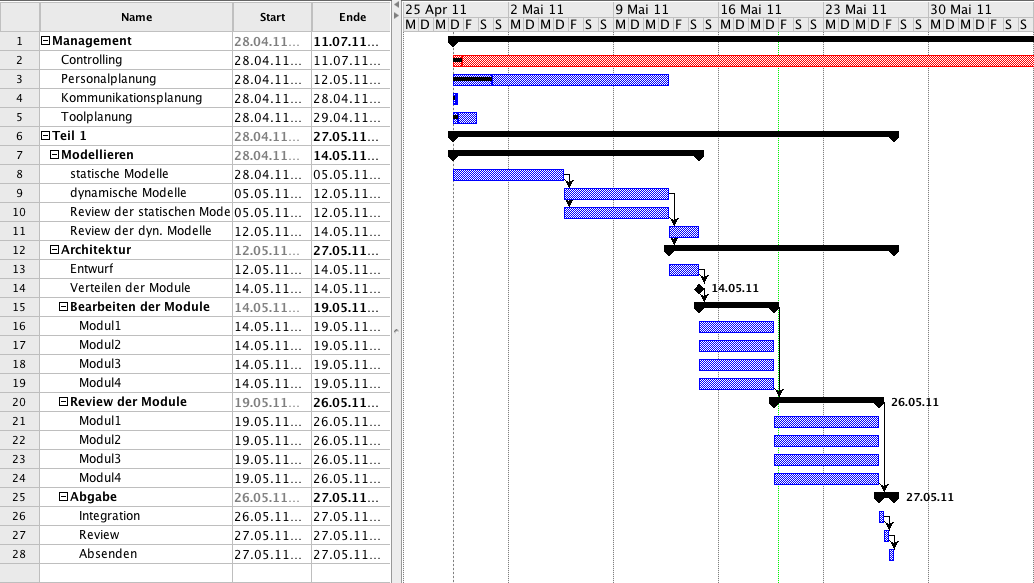
\includegraphics{data/fig/ganth_beispiel.png}}
Die Managementattribute des Softwareprodukts und dessen Anforderungen, werden anfangs mit Initialwerten samt Wertebereich versehen:\\
\ \\
Priorität aus Auftraggebersicht = {hoch, mittel, niedrig}\\
Priorität aus Auftragnehmersicht = {hoch, mittel, niedrig}\\
Stabilität = {fest, gefestigt, volatil}\\
Kritikalität = {hoch, mittel, niedrig, keine}\\
Entwicklungsrisiko = {hoch, mittel, niedrig}\\

\subsection{Dokumentationsattribute}
Autor	
Eindeutige Teamnummer	
Quelle	
Version	
Bearbeitungsstatus	

\subsection{Managementsattribute}
\begin{itemize}
	\item[] Managementattribute
	\item[] Priorität
	\item[]	Stabilität
	\item[] Kritikalität	
	\item[] Entwicklungsrisiko
\end{itemize}



\section{Visionen und Ziele}

	\noindent 	
%%%%%%%%%%%%%%%%%%%%%%%%%%%%%%%%%%%%%%%
%                                                                              
% 		Visionen und Ziele			      		
%                                                                              
%%%%%%%%%%%%%%%%%%%%%%%%%%%%%%%%%%%%%%%
Verfeinern Sie hier die Visionen und Ziele, die im Lastenheft definiert wurden. Falls kein Lastenheft vorliegt, definieren Sie Ihre Visionen und Ziele.

Verwenden Sie die folgenden Kürzel, um Ihre Visionen und Ziele eindeutig zu identifizieren.
/PV10/ für die erste Vision
/PV20/ für die zweite Vision
usw.

/Pz10/ für die erste Ziele
/PZ20/ für die zweite Ziele
	
\section{Rahmenbedingungen}

	\noindent %%%%%%%%%%%%%%%%%%%%%%%%%%%%%%%%%%%%%%%
%                                                                              
% 		Rahmenbedingungen			      		
%                                                                              
%%%%%%%%%%%%%%%%%%%%%%%%%%%%%%%%%%%%%%%
Beschreiben Sie hier Anwendungsbereiche, Zielgruppen und Betriebsbedingungen des Softwareprodukts (etwa Hardware, Software, Betriebszeit oder Schnittstellen).\\

Verwenden Sie die folgenden Kürzel, um Ihre Rahmenbedingungen eindeutig zu identifizieren.
/PR10/ für die erste Rahmenbedingung
/PR20/ für die zweite Rahmenbedingung
usw.

	
\section{Kontext und Überblick}

	\noindent %%%%%%%%%%%%%%%%%%%%%%%%%%%%%%%%%%%%%%%
%                                                                              
% 		Kontext und Überblick		      		
%                                                                              
%%%%%%%%%%%%%%%%%%%%%%%%%%%%%%%%%%%%%%%	

Die relevante Systemumgebung (Kontext) und Überblick über das Softwareprodukt.

Verwenden Sie die folgenden Kürzel, um Ihre Kontextelemente eindeutig zu identifizieren.
/PK10/ für den ersten Kontext
/PK20/ für den ersten Kontext
usw.

	
\section{Anforderungen}

	\noindent %%%%%%%%%%%%%%%%%%%%%%%%%%%%%%%%%%%%%%%
%                                                                              
% 		Anforderungen		      		
%                                                                              
%%%%%%%%%%%%%%%%%%%%%%%%%%%%%%%%%%%%%%%

\subsection{Funktionale Anforderungen}
Beschreibung des Softwareprodukts aus Auftraggebersicht und auf oberster Abstraktionsebene; keine Detailbeschreibungen!

Verwenden Sie die folgenden Kürzel, um Ihre Anforderungen eindeutig zu identifizieren.
/PF10/ für die erste funktionale Anforderung
/PF20/ für die zweite funktionale Anforderung
usw.

\subsection{Nicht-Funktionale Anforderungen}

Qualitätsanforderungen
Qualitätsziele anhand einer Tabelle bestimmen, wie unten angeführt:\\

         TODO Tabelle mit Rahmen recherchieren\\
         \ \\
        \begin{tabularx}{\textwidth}{ l l l l l }
            \emph{Systemqualität} & \emph{Sehr gut} & \emph{Gut}& \emph{Normal} & \emph{Nicht relevant}\\
            
			Funktionalität	& & X & &\\
			
			Zuverlässigkeit	& X & & &\\

			Benutzbarkeit	& & X & &\\

			Effizienz		& & & X &\\

			Wartbarkeit		& & & X &\\

			Portabilität		& & & X &\\

        \end{tabularx}
           
\ \\
Tabelle 1: Qualitätsanforderungen\\

Die in Tabelle 1 angegebenen Bewertungen sind nur beispielhaft gewählt.
Eine Verfeinerung der in der Tabelle genannten Qualitätsmerkmale finden sich in der ISO/IEC 9126-1. Je nach Größe des Projekts können Sie mit der o.g. Tabelle arbeiten oder Verfeinerungen angeben.

Verwenden Sie z.B. die folgenden Kürzel, um Ihre Qualitätsanforderungen eindeutig zu identifizieren:
\begin{itemize}
	\item /PQBE10/ für die erste Qualitätsanforderung zur Benutzbarkeit (Erlernbarkeit)
	\item[]für die erste Qualitätsanforderung zur Wartbarkeit (Stabilität)
\end{itemize}
	
	
\section{Abnahmekriterien}

	\noindent %%%%%%%%%%%%%%%%%%%%%%%%%%%%%%%%%%%%%%%
%                                                                              
% 		Abnahmekriterien		      		
%                                                                              
%%%%%%%%%%%%%%%%%%%%%%%%%%%%%%%%%%%%%%%
Legen Sie hier die Kriterien fest, die bei Abnahme das Produkt auf Realisierung/Erfüllung der Anforderungen prüfen. Sie können hier u.a. Testfälle (definiert in Testklassen) angeben oder darauf verweisen, die die Erfüllung Ihrer Anforderungen überprüfen. Definieren Sie diesen Abschnitt möglichst vor der Implementierung.
	
				
\section{Subsystemstruktur}

	\noindent Subsystemstruktur (optional)
Gliedern Sie hier die Stufen der Entwicklung die Ihr Softwareprodukt durchlaufen soll.

				
\section{Glossar}

	\noindent Glossar
Führen Sie hier Glossarbegriffe mit Erklärungen auf; Verweise auf andere Glossarbegriffe werden mit einem Pfeil (/Begriff) gekennzeichnet. Synonyme und Übersetzungen werden in Klammern hinter dem Begriff vermerkt.
	
	
\section{Literatur}

	\noindent Literatur\\

Wenn Sie Literatur oder andere Quellen verwendet haben, dann führen Sie diese in diesem Abschnitt auf und verweisen an entsprechender Stelle in diesem Dokument darauf.
\subsection{Hinweis zu dieser Vorlage}
Die Vorlage für dieses Pflichtenheft wurde Balzert (2009), S. 492 ff. entnommen.
\subsection{Literaturliste}
Balzert, Helmut (2009). Lehrbuch der Softwaretechnik: Basiskonzepte und Requirements Engineering. 3. Auflage. Heidelberg: Spektrum, Seite 492 ff.




\end{document}